\chapter*{引言}
\phantomsection
\addcontentsline{toc}{chapter}{引言}

本卷的目的在于初等地研究单个实变量的无穷小性质；把这些性质推广到多个实变量的函数，更不必说定义在更一般空间上的函数，将只在以后的诸卷中处理。

我们将证明的结果首先对于实变量的（有限）实值函数有用；但其中大多数无需进一步的论证便可推广到取值于 R 上的拓扑向量空间的实变函数（见下文）；由于这类函数在分析中经常出现，我们将对它们陈述所有并非实值函数所特有的结果。

我们刚才谈到的拓扑向量空间这一概念，在本丛书的第 V 卷中有定义并详加研究；但本卷并不需要第 V 卷的任何结果；不过需要其中的一些定义，为方便读者起见，我们在下面把它们复述出来。

我们不再重复（交换）域 K 上的向量空间的定义（Alg., II, p.~193）。\(^{1}\) 拓扑域 K 上的拓扑向量空间 E 是指 K 上的一个向量空间，带有一个拓扑，使得函数 \(x + y\) 和 xt 分别在 \(E \times E\) 与 \(E \times K\) 上连续；特别地，这样的拓扑与 E 的加法群结构相容。本卷中所考虑的拓扑向量空间都默认为豪斯多夫空间。当拓扑群 E 完备时，就称拓扑向量空间 E 是完备的。赋值域 K 上的每个赋范向量空间（Gen.~Top., IX, p.~169） \(^{2}\) 都是 K 上的拓扑向量空间。

设 E 是实数域 R 上的一个向量空间（带拓扑或不带拓扑）；若 x、y 是 E 中任意两点，则点 \(\mathbf{x}t + \mathbf{y}(1 - t)\) （t 跑遍 R 中的闭线段 {[}0, 1{]} ）所成的集合称为以 x、y 为端点的闭线段。若对于 A 中任意两点 x、y，以 x 和 y 为端点的闭线段都包含于 A 中，则称 E 的子集 A 是凸的。例如，仿射线性簇是凸的；任一闭线段也是凸的；在 \(R^{n}\) 中，任何超平行体（Gen.~Top., VI, p.~34）都是凸的。凸集的任意交是凸的。

我们称域 R 上的拓扑向量空间 E 是局部凸的，如果原点（从而 E 的每一点）具有由凸邻域组成的基本邻域系。每个赋范空间都是局部凸的；事实上，球 \(\|x\| \leqslant r (r > 0)\) 构成 E 中 0 的一个基本邻域系，而且其中每个球都是凸的，因为关系式 \(\|x\| \leqslant r\) 与 \(\|y\| \leqslant r\) 蕴含

\[
\| \mathbf {x} t + \mathbf {y} (1 - t) \| \leqslant \| \mathbf {x} \| t + \| \mathbf {y} \| (1 - t) \leqslant r
\]

对 \(0 \leqslant t \leqslant 1\) 成立。

最后，(交换) 拓扑域 K 上的拓扑代数 A 是指 K 上的一个代数，带有一个拓扑，使得函数 \(x + y\) 、xy 与 xt 分别在 \(A \times A\) 、 \(A \times A\) 与 \(A \times K\) 上连续；当只给 A 赋予其拓扑及其 K 上的向量空间结构时，A 便是一个拓扑向量空间。赋值域 K 上的每个赋范代数（Gen.~Top., IX, p.~175）都是 K 上的拓扑代数。

\chapter{导数}

\section{一阶导数}

正如引言中所说，在本章及下一章中，我们将研究定义在实数域 \(\mathbf{R}\) 的子集上、取值于一个豪斯多夫拓扑向量空间 \(E\) （在域 \(\mathbf{R}\) 上）中的函数的无穷小性质；为简便起见，我们称这种函数为实变向量函数。最重要的情形是 \(E = \mathbf{R}\) （实变量的实值函数）的情形。当 \(E = \mathbf{R}^n\) 时，对取值于 \(E\) 中的向量函数的考虑可化为对 \(n\) 个有限实函数的同时考虑。

第一章中陈述的许多定义和性质可以推广到定义在复数域 C 的子集上、取值于 C 上的拓扑向量空间中的函数（复变向量函数）。其中一些定义和性质甚至可以推广到定义在任意交换拓扑域 K 的子集上、取值于 K 上的拓扑向量空间中的函数。

我们将在行文中顺带指出这些推广（特别参见 I, p.~10 的注 2），而把重点放在复变函数的情形上，它连同实变函数一起显然是最重要的，并将在本丛书稍后的一卷中得到更深入的研究。

\subsection{向量函数的导数}

定义 1. 设 \(\mathbf{f}\) 是定义在一个不退化为一点的区间 \(\mathbf{I} \subset \mathbf{R}\) 上的向量函数。我们说 \(\mathbf{f}\) 在一点 \(x_0 \in \mathbf{I}\) 处可导，如果

\(\lim_{x\to x_{0},x\in I,x\neq x_{0}}\frac{\mathbf{f}(x)-\mathbf{f}(x_{0})}{x-x_{0}}\) 存在（在 f 取值的那个向量空间中）；这个

极限的值称为 f 在点 \(x_{0}\) 处的一阶导数（或简称导数），记作 \(\mathbf{f}'(x_{0})\) 或 \(\mathbf{D}\mathbf{f}(x_{0})\) 。

若 f 在点 \(x_{0}\) 可导，则 f 在任何区间 \(J \subset I\) （不退化为一点且使 \(x_{0} \in J\) ）上的限制也可导，且这限制的导数等于 \(\mathbf{f}'(x_{0})\) 。反之，设 J 是含于 I 且包含 \(x_{0}\) 相对于 I 的一个邻域的区间；若 f 在 J 上的限制在点 \(x_{0}\) 处有导数，则 f 亦然。

我们把这些性质概括为一句话：导数概念是一个局部概念。

注。*1) 在运动学中，若点 \(\mathbf{f}(t)\) 是动点在空间 \(\mathbf{R}^3\) 中在时刻 \(t\) 的位置，则 \(\frac{\mathbf{f}(t) - \mathbf{f}(t_0)}{t - t_0}\) 称为时刻 \(t_0\) 与 \(t\) 之间的平均速度，而其极限 \(\mathbf{f}'(t_0)\) 是时刻 \(t_0\) 的瞬时速度（或简称速度）（当此极限存在时）。*

\begin{enumerate}
\def\labelenumi{\arabic{enumi})}
\setcounter{enumi}{1}
\tightlist
\item
  若定义在 I 上的函数 \(\mathbf{f}\) 在一点 \(x_0 \in I\) 处可导，则它在该点必相对于 I 连续。
\end{enumerate}

定义 2. 设 \(\mathbf{f}\) 是定义在区间 \(\mathrm{I} \subset \mathbf{R}\) 上的向量函数，并设 \(x_0\) 是 \(\mathrm{I}\) 中使区间 \(\mathrm{I} \cap [x_0, +\infty[\) （相应地，\(\mathrm{I} \cap ] - \infty, x_0]\) ）不退化为一点的点。若 \(\mathbf{f}\) 在点 \(x_0\) 右可导（相应地，左可导），指的是：\(\mathbf{f}\) 在区间 \(\mathrm{I} \cap [x_0, +\infty[\) （相应地，\(\mathrm{I} \cap ] - \infty, x_0]\) ）上的限制在点 \(x_0\) 可导；这一限制在点 \(x_0\) 的导数值称为 \(\mathbf{f}\) 在点 \(x_0\) 的右导数（相应地，左导数），记作 \(\mathbf{f}_d'(x_0)\) （相应地，\(\mathbf{f}_g'(x_0)\) ）。

设 f 是定义在 I 上的向量函数，\(x_{0}\) 是 I 的一个内点且 f 在该点连续；由定义 1 和 2 可知，f 在 \(x_{0}\) 可导当且仅当 f 在该点既有右导数又有左导数，且这两个导数相等；此时

\[
\mathbf {f} ^ {\prime} (x _ {0}) = \mathbf {f} _ {d} ^ {\prime} (x _ {0}) = \mathbf {f} _ {g} ^ {\prime} (x _ {0}).
\]

例。1) 常函数在每一点的导数都为零。

\begin{enumerate}
\def\labelenumi{\arabic{enumi})}
\setcounter{enumi}{1}
\item
  仿射线性函数 \(x \mapsto ax + b\) 在每一点的导数都等于 a。
\item
  实函数 \(1 / x\) （对 \(x \neq 0\) 有定义）在每个点 \(x_0 \neq 0\) 处可导，因为我们有 \(\left(\frac{1}{x} - \frac{1}{x_0}\right) / (x - x_0) = -\frac{1}{xx_0}\) ，而且由于 \(1 / x\) 在 \(x_0\) 连续，前述表达式的极限为 \(-1 / x_0^2\) 。
\item
  数量函数 \(|x|\) 定义在 \(\mathbf{R}\) 上，它具有右导数 \(+1\) 与左导数 \(-1\) （在 \(x = 0\) 处）；它在该点不可导。
\end{enumerate}

*5) 实函数在 \(x = 0\) 时等于 0、等于 \(x \sin 1/x\) （当 \(x \neq 0\) ），它在 \(\mathbf{R}\) 上有定义且连续，但在点 \(x \neq 0\) 处既无右导数亦无左导数。可以给出在区间上连续而在区间每一点都没有导数的函数的例子（I, p.~35, exerc. 2 和 3）。

定义 3. 设 \(\mathbf{f}\) 是定义在区间 \(\mathrm{I} \subset \mathbf{R}\) 上的向量函数；若它在 \(\mathrm{I}\) 的每一点可导（相应地，右可导、左可导），则称它在 \(\mathrm{I}\) 上可导（相应地，右可导、左可导）；函数 \(x \mapsto \mathbf{f}'(x)\) （相应地，\(x \mapsto \mathbf{f}_d'(x)\) 、\(x \mapsto \mathbf{f}_g'(x)\) ）定义在 \(\mathrm{I}\) 上，称为 \(\mathbf{f}\) 的导函数，或（滥用语言的说法）导数（相应地，右导数、左导数），记作 \(\mathbf{f}'\) 或 \(\mathrm{Df}\) 或 \(df/dx\) （相应地，\(\mathbf{f}_d', \mathbf{f}_g'\) ）。

注。一个函数可以在某个区间上可导，而其导数不必在区间的每一点连续（cf.~I, p.~36, exerc. 5）；*在 x = 0 时等于 0、等于 \(x^{2} \sin 1/x\) （当 \(x \neq 0\) ）的函数的例子就表明了这一点；它处处有导数，但这导数在点 \(x = 0\) 不连续*

\subsection{求导的线性性}

命题 1. 定义在区间 \(I \subset R\) 上、取值于给定的拓扑向量空间 E 中、且在点 \(x_{0}\) 可导的向量函数所成的集是 R 上的一个向量空间，且映射 \(\mathbf{f} \mapsto \mathrm{Df}(x_{0})\) 是从此空间到 E 中的线性映射。

换句话说，若 f 和 g 定义在 I 上且在点 \(x_{0}\) 可导，则 \(f + g\) 与 fa（a 为任意标量）在 \(x_{0}\) 可导，且它们在那里的导数分别是 \(\mathbf{f}'(x_{0}) + \mathbf{g}'(x_{0})\) 与 \(\mathbf{f}'(x_{0})a\) 。这由 \(x + y\) 及 xa 在 E × E 与 E 上的连续性立即得出。

推论. 定义在区间 I 上、取值于给定的拓扑向量空间 E 中、且在 I 上可导的向量函数所成的集是 R 上的向量空间，且映射 \(f \mapsto Df\) 是从此空间到从 I 到 E 的映射所成的向量空间中的线性映射。

注. 若对从 I 到 E 的映射所成的向量空间及其可导映射组成的子空间（cf.~Gen.~Top., X, p.~277）赋予简单收敛拓扑（或一致收敛拓扑），则线性映射 \(\mathbf{f} \mapsto \mathrm{Df}\) （一般）不连续*例如，函数序列 \(\mathbf{f}_n(x) = \sin n^2 x / n\) 在 \(\mathbf{R}\) 上一致收敛于 0，但导数序列 \(\mathbf{f}_n'(x) = n\cos n^2 x\) 甚至不简单收敛于 \(0\)*

命题 2. 设 E 和 F 是 R 上的两个拓扑向量空间，u 是从 E 到 F 中的连续线性映射。若 f 是定义在区间 \(I \subset R\) 上、取值于 E 中、且在点 \(x_{0} \in I\) 可导的向量函数，则复合函数 \(u \circ f\) 具有导数，等于 \(\mathbf{u}(\mathbf{f}'(x_{0}))\) （在 \(x_{0}\) 处）。

事实上，由于 \(\frac{\mathbf{u}(\mathbf{f}(x)) - \mathbf{u}(\mathbf{f}(x_0))}{x - x_0} = \mathbf{u}\left(\frac{\mathbf{f}(x) - \mathbf{f}(x_0)}{x - x_0}\right)\) ，结论由 \(\mathbf{u}\) 的连续性得出。

推论. 若 \(\varphi\) 是 \(E\) 上的连续线性形式，则实函数 \(\varphi \circ \mathbf{f}\) 具有导数，等于 \(\varphi(\mathbf{f}'(x_0))\) （在点 \(x_0\) 处）。

例。1) 设 \(\mathbf{f} = (f_i)_{1\leqslant i\leqslant n}\) 是取值于 \(\mathbf{R}^n\) 中、定义在区间 \(I\subset \mathbf{R}\) 上的函数；每个实函数 \(f_{i}\) 无非是复合函数 \(\mathrm{pr}_i\circ \mathbf{f}\) ，故它在点 \(x_0\) 与 \(\mathbf{f}\) 同时可导，且此时 \(\mathbf{f}'(x_0) = (f_i'(x_0))_{1\leqslant i\leqslant n}\) 。

*2) 在运动学中，若 \(\mathbf{f}(t)\) 是动点 M 在时刻 \(t\) 的位置，\(\mathbf{g}(t)\) 是 M 在平面 P（相应地，直线 D）上的投影 \(\mathbf{M}'\) 在同一时刻的位置，而投影的核是与 P（相应地，D）不平行的一条直线（相应地，一个平面），则 \(\mathbf{g}\) 是投影 \(\mathbf{u}\) （从 \(\mathbf{R}^3\) 到 P（相应地，D）上）与 \(\mathbf{f}\) 的复合；由于 \(\mathbf{u}\) 是（连续）线性映射，可见动点的速度在平面（相应地，直线）上的投影等于该动点在此平面（相应地，直线）上投影的速度。*

\begin{enumerate}
\def\labelenumi{\arabic{enumi})}
\setcounter{enumi}{2}
\tightlist
\item
  设 \(f\) 是定义在区间 \(\mathbf{I} \subset \mathbf{R}\) 上的复值函数，\(a\) 为任意复数；命题 2 表明，若 \(f\) 在一点 \(x_0\) 可导，则 \(af\) 也可导，且此函数在 \(x_0\) 的导数等于 \(af'(x_0)\) 。
\end{enumerate}

\subsection{乘积的导数}

现在考虑 \(p\) 个拓扑向量空间 \(\mathrm{E}_i\) （ \(1 \leqslant i \leqslant p\) ，在 \(\mathbf{R}\) 上），以及一个连续多线性 \(^1\) 映射（我们将把它记作

\[
\left(\mathbf {x} _ {1}, \mathbf {x} _ {2}, \dots , \mathbf {x} _ {p}\right) \mapsto \left[ \mathbf {x} _ {1}. \mathbf {x} _ {2} \dots \mathbf {x} _ {p} \right])
\]

它把 \(E_{1} \times E_{2} \times \cdots \times E_{p}\) 映入 R 上的一个拓扑向量空间 F 中。

命题 3. 对每个指标 \(i\) ( \(1 \leqslant i \leqslant p\) )，设 \(\mathbf{f}_i\) 是定义在区间 \(\mathrm{I} \subset \mathbf{R}\) 上、取值于 \(\mathrm{E}_i\) 中、且在点 \(x_0 \in \mathrm{I}\) 可导的函数。则函数

\[
x \mapsto [ \mathbf {f} _ {1} (x). \mathbf {f} _ {2} (x) \dots \mathbf {f} _ {p} (x) ]
\]

定义在 I 上、取值于 F 中，它具有导数，等于

\[
\sum_ {i = 1} ^ {p} \left[ \mathbf {f} _ {1} (x _ {0}) \dots \mathbf {f} _ {i - 1} (x _ {0}). \mathbf {f} _ {i} ^ {\prime} (x _ {0}). \mathbf {f} _ {i + 1} (x _ {0}) \dots \mathbf {f} _ {p} (x _ {0}) \right]\tag{1}
\]

（在点 \(x_0\) 处）。

令 \(\mathbf{h}(x) = [\mathbf{f}_1(x).\mathbf{f}_2(x)\dots \mathbf{f}_p(x)]\) ；则由恒等式

\[
\left[ \mathbf {b} _ {1}. \mathbf {b} _ {2} \dots \mathbf {b} _ {p} \right] - \left[ \mathbf {a} _ {1}. \mathbf {a} _ {2} \dots \mathbf {a} _ {p} \right] = \sum_ {i = 1} ^ {p} \left[ \mathbf {b} _ {1} \dots \mathbf {b} _ {i - 1}. (\mathbf {b} _ {i} - \mathbf {a} _ {i}). \mathbf {a} _ {i + 1} \dots \mathbf {a} _ {p} \right],
\]

我们便可写出

\[
\mathbf {h} (x) - \mathbf {h} (x _ {0}) = \sum_ {i = 1} ^ {p} \left[ \mathbf {f} _ {1} (x) \dots \mathbf {f} _ {i - 1} (x). (\mathbf {f} _ {i} (x) - \mathbf {f} _ {i} (x _ {0})). \mathbf {f} _ {i + 1} (x _ {0}) \dots \mathbf {f} _ {p} (x _ {0}) \right].
\]

把等式两边同乘 \(\frac{1}{x - x_0}\) 并让 \(x\) 在 I 中趋于 \(x_0\) ，便得到表达式 (1)，因为映射

\[
(\mathbf {x} _ {1}, \mathbf {x} _ {2}, \dots , \mathbf {x} _ {p}) \mapsto [ \mathbf {x} _ {1}. \mathbf {x} _ {2} \dots \mathbf {x} _ {p} ]
\]

与 F 中的加法都是连续的。

\(^{1}\) 回忆（Alg., II, p.~265）下面的定义：如果从 \(E_{1} \times E_{2} \times \cdots \times E_{p}\) 到 F 中的映射 f 的每个偏映射

\[
\mathbf {x} _ {i} \mapsto \mathbf {f} (\mathbf {a} _ {1}, \dots , \mathbf {a} _ {i - 1}, \mathbf {x} _ {i}, \mathbf {a} _ {i + 1}, \dots , \mathbf {a} _ {p})
\]

从 \(E_{i}\) 到 F （ \(1 \leqslant i \leqslant p\) ）都是线性映射，其中 \(a_{j}\) （对于 \(j \neq i\) 的下标）在 \(E_{j}\) 中任意取定，则称 f 是多线性的。我们指出，若诸 \(E_{i}\) 在 R 上有限维，则从 \(E_{1} \times E_{2} \times \cdots \times E_{p}\) 到 F 中的每个多线性映射必定连续；当这些空间中有一些是无穷维拓扑向量空间时，则未必如此。

当某些函数 \(\mathbf{f}_i\) 为常数时，表达式 (1) 中含有其导数 \(\mathbf{f}_i'(x_0)\) 的项为零。

我们详细考察应用中最重要的特例 \(p = 2\) ：若 \((\mathbf{x}, \mathbf{y}) \mapsto [\mathbf{x}.\mathbf{y}]\) 是 \(\mathrm{E} \times \mathrm{F}\) 到 \(\mathrm{G}\) 中的连续双线性映射（E、F、G 为 \(\mathbf{R}\) 上的拓扑向量空间），而 \(\mathbf{f}\) 和 \(\mathbf{g}\) 是两个向量函数，分别在点 \(x_0\) 可导，各取值于 E 和 F 中，则向量函数 \(x \mapsto [\mathbf{f}(x).\mathbf{g}(x)]\) （我们把它记作 \([\mathbf{f}.\mathbf{g}]\) ）具有导数，等于 \([\mathbf{f}'(x_0).\mathbf{g}(x_0)] + [\mathbf{f}(x_0).\mathbf{g}'(x_0)]\) （在 \(x_0\) 处）。特别地，若 \(\mathbf{a}\) 是常向量，则 \([\mathbf{a}.\mathbf{f}]\) （相应地，\([\mathbf{f}.\mathbf{a}]\) ）具有导数，等于 \([\mathbf{a}.\mathbf{f}'(x_0)]\) （相应地，\([\mathbf{f}'(x_0).\mathbf{a}]\) ）（在 \(x_0\) 处）。

若 \(\mathbf{f}\) 和 \(\mathbf{g}\) 都在 I 上可导，则 {[}f.g{]} 也在 I 上可导，且我们有

\[
\left[ \mathbf {f}. \mathbf {g} \right] ^ {\prime} = \left[ \mathbf {f} ^ {\prime}. \mathbf {g} \right] + \left[ \mathbf {f}. \mathbf {g} ^ {\prime} \right].\tag{2}
\]

例。1) 设 \(f\) 是实函数，\(\mathbf{g}\) 是向量函数，二者都在点 \(x_0\) 可导；函数 \(\mathbf{g}f\) 具有导数，等于 \(\mathbf{g}'(x_0)f(x_0) + \mathbf{g}(x_0)f'(x_0)\) （在 \(x_0\) 处）。特别地，若 \(\mathbf{a}\) 为常数，则 \(\mathbf{a}f\) 具有导数 \(\mathbf{a}f'(x_0)\) 。最后这个注记结合 I, p.~5 的例 1 证明：若 \(\mathbf{f} = (f_i)_{1 \leqslant i \leqslant n}\) 是取值于 \(\mathbf{R}^n\) 中的向量函数，则 \(\mathbf{f}\) 在点 \(x_0\) 可导当且仅当每个实函数 \(f_i\) ( \(1 \leqslant i \leqslant n\) ) 都在该点可导：因为若 \((\mathbf{e}_i)_{1 \leqslant i \leqslant n}\) 是 \(\mathbf{R}^n\) 的规范基，我们便可写 \(\mathbf{f} = \sum_{i=1}^{n} \mathbf{e}_i f_i\) 。

\begin{enumerate}
\def\labelenumi{\arabic{enumi})}
\setcounter{enumi}{1}
\tightlist
\item
  实函数 \(x^{n}\) 得自多线性函数
\end{enumerate}

\[
(x _ {1}, x _ {2}, \ldots , x _ {n}) \mapsto x _ {1} x _ {2} \ldots x _ {n}
\]

它定义在 \(R^{n}\) 上，是通过把每个 \(x_{i}\) 都换成 x 而得到的；于是命题 3 表明 \(x^{n}\) 在 R 上可导且具有导数 \(nx^{n-1}\) 。由此，多项式函数 \(a_{0}x^{n} + a_{1}x^{n-1} + \cdots + a_{n-1}x + a_{n}\) （诸 \(a_{i}\) 为常向量）具有导数

\[
n \mathbf {a} _ {0} x ^ {n - 1} + (n - 1) \mathbf {a} _ {1} x ^ {n - 2} + \dots + \mathbf {a} _ {n - 1};
\]

当诸 \(\mathbf{a}_i\) 为实数时，此函数与代数学（A, IV）中所定义的多项式函数的导数相一致。

\begin{enumerate}
\def\labelenumi{\arabic{enumi})}
\setcounter{enumi}{2}
\tightlist
\item
  欧氏数量积 \((\mathbf{x}|\mathbf{y})\) (Gen.~Top., VI, p.~40) 是 \(R^{n}\times R^{n}\) 到 R 中的一个双线性映射（必然连续）。若 f 和 g 是取值于 \(R^{n}\) 、且在点 \(x_{0}\) 可导的两个向量函数，则实函数 \(x\mapsto(\mathbf{f}(x)|\mathbf{g}(x))\) 具有导数，等于 \((\mathbf{f}'(x_{0})|\mathbf{g}(x_{0}))+(\mathbf{f}(x_{0})|\mathbf{g}'(x_{0}))\) （在点 \(x_{0}\) 处）。对 \(C^{n}\) 上的埃尔米特数量积有类似的结果，这时把该空间看作 R 上的向量空间。
\end{enumerate}

我们特别考察欧氏范数 \(\|\mathbf{f}(x)\|\) 为常数的情形，此时 \((\mathbf{f}(x) \mid \mathbf{f}(x)) = \|\mathbf{f}(x)\|^{2}\) 也是常数；写出 \((\mathbf{f}(x) \mid \mathbf{f}(x))\) 的导数在 \(x_{0}\) 处为零，便得到 \((\mathbf{f}(x_{0}) \mid \mathbf{f}'(x_{0})) = 0\) ；换句话说，\(\mathbf{f}'(x_{0})\) 与 \(\mathbf{f}(x_{0})\) 正交。

\begin{enumerate}
\def\labelenumi{\arabic{enumi})}
\setcounter{enumi}{3}
\item
  若 E 是 R 上的一个拓扑代数（cf.~Introduction），E 的两个元素之积 xy 便是 \((\mathbf{x}, \mathbf{y})\) 的连续双线性函数；若 f 与 g 取值于 E 且在点 \(x_{0}\) 可导，则函数 \(x \mapsto \mathbf{f}(x)\mathbf{g}(x)\) 具有导数，等于 \(\mathbf{f}'(x_{0})\mathbf{g}(x_{0}) + \mathbf{f}(x_{0})\mathbf{g}'(x_{0})\) （在 \(x_{0}\) 处）。特别地，若 \(U(x) = (\alpha_{ij}(x))\) 与 \(V(x) = (\beta_{ij}(x))\) 是两个 n 阶方阵，在 \(x_{0}\) 可导，则其乘积 UV 具有导数，等于 \(U'(x_{0})V(x_{0}) + U(x_{0})V'(x_{0})\) （在 \(x_{0}\) 处）（其中 \(U'(x) = (\alpha'_{ij}(x))\) ，\(V'(x) = (\beta'_{ij}(x)))\) 。
\item
  行列式 \(\operatorname{det}(\mathbf{x}_1, \mathbf{x}_2, \ldots, \mathbf{x}_n)\) （\(n\) 个向量 \(\mathbf{x}_i = (x_{ij})_{1 \leqslant j \leqslant n}\) 的行列式，这些向量取自空间 \(\mathbf{R}^n\) ；Alg., III, p.~522）既然是诸 \(\mathbf{x}_i\) 的（连续）多线性函数，便可以看出：若 \(n^2\) 个实函数 \(f_{ij}\) 都在 \(x_0\) 可导，则它们的行列式 \(g(x) = \det(f_{ij}(x))\) 具有导数，等于
\end{enumerate}

\[
\sum_ {i = 1} ^ {n} \left[ \mathbf {f} _ {1} (x _ {0}), \dots , \mathbf {f} _ {i - 1} (x _ {0}), \mathbf {f} _ {i} ^ {\prime} (x _ {0}), \mathbf {f} _ {i + 1} (x _ {0}), \dots , \mathbf {f} _ {n} (x _ {0}) \right]
\]

（在 \(x_{0}\) 处），其中 \(\mathbf{f}_{i}(x)=(f_{ij}(x))_{1\leqslant j\leqslant n}\) ；换句话说，对每个 i，把 n 阶行列式中第 \(i^{th}\) 列的元素换成它们的导数，这样形成的 n 个行列式之和便是该行列式的导数。

注. 若 \(U(x)\) 是在点 \(x_{0}\) 可导且可逆的方阵，则其行列式 \(\Delta(x) = \det(U(x))\) 的导数可通过 \(U(x)\) 的导数由公式

\[
\varDelta^ {\prime} (x _ {0}) = \varDelta (x _ {0}). \mathrm{Tr} (U ^ {\prime} (x _ {0}) U ^ {- 1} (x _ {0})).\tag{3}
\]

表出。事实上，令 \(U(x_0 + h) = U(x_0) + hV\) ；则按定义，\(V\) 趋于 \(U'(x_0)\) （当 \(h\) 趋于 0 时）。可以写出

\[
\Delta (x _ {0} + h) = \Delta (x _ {0}). \det (I + h V U ^ {- 1} (x _ {0})).
\]

现在 \(\det(I + hX) = 1 + h\operatorname{Tr}(X) + \sum_{k=2}^{n} \lambda_k h^k\) ，其中 \(\lambda_k (k \geqslant 2)\) 是矩阵 X 的元素的多项式；由于当 h 趋于 0 时 \(VU^{-1}(x_0)\) 的元素有极限，我们确实得到公式 (3)。

\subsection{函数逆元的导数}

命题 4. 设 E 是 R 上具有单位元的完备赋范代数，设 f 是定义在区间 I ⊂ R 上、取值于 E 中、且在点 \(x_{0} \in I\) 可导的函数。若 \(\mathbf{y}_{0} = \mathbf{f}(x_{0})\) 在 E 中可逆 \(^{2}\) ，则函数 \(x \mapsto (\mathbf{f}(x))^{-1}\) 在 \(x_{0}\) 的（相对于 I 的）一个邻域上有定义，且具有导数，等于 \(-\left(\mathbf{f}(x_{0})\right)^{-1}\mathbf{f}'(x_{0})\left(\mathbf{f}(x_{0})\right)^{-1}\) （在 \(x_{0}\) 处）。

事实上，E 中可逆元所成的集是一个开集，函数 \(y \mapsto y^{-1}\) 在其上连续（Gen.~Top., IX, p.~178）；由于 f 在 \(x_{0}\) （相对于 I）连续，\(\left(\mathbf{f}(x)\right)^{-1}\) 在 \(x_{0}\) 的一个邻域上有定义，且我们有

\[
\left(\mathbf {f} (x)\right) ^ {- 1} - \left(\mathbf {f} \left(x _ {0}\right)\right) ^ {- 1} = \left(\mathbf {f} (x)\right) ^ {- 1} \left(\mathbf {f} \left(x _ {0}\right) - \mathbf {f} (x)\right) \left(\mathbf {f} \left(x _ {0}\right)\right) ^ {- 1}.
\]

于是命题由 \(y^{-1}\) 在 \(y_{0}\) 的一个邻域上的连续性以及 xy 在 \(E \times E\) 上的连续性得出。

例。1) 最重要的特例是 E 为域 R 或 C 之一的情形：若 f 是实值或复值函数，在点 \(x_{0}\) 可导且 \(f(x_{0}) \neq 0\) ，则 1/f 具有导数，等于 \(-f'(x_{0})/(f(x_{0}))^{2}\) （在 \(x_{0}\) 处）。

\begin{enumerate}
\def\labelenumi{\arabic{enumi})}
\setcounter{enumi}{1}
\tightlist
\item
  若 \(U = (\alpha_{ij}(x))\) 是 n 阶方阵，在 \(x_{0}\) 可导且在该点可逆，则 \(U^{-1}\) 具有导数，等于 \(-U^{-1}U'U^{-1}\) （在 \(x_{0}\) 处）。
\end{enumerate}

\subsection{复合函数的导数}

命题 5. 设 f 是定义在区间 \(I \subset R\) 上的实函数，g 是定义在 R 的一个包含 \(f(I)\) 的区间上的向量函数。若 f 在点 \(x_{0}\) 可导且 g 在点 \(f(x_{0})\) 可导，则复合函数 \(g \circ f\) 具有导数，等于 \(\mathbf{g}'(f(x_{0}))f'(x_{0})\) （在 \(x_{0}\) 处）。

令 \(\mathbf{h} = \mathbf{g} \circ f\) ；对 \(x \neq x_0\) 我们可以写出

\[
\frac {\mathbf {h} (x) - \mathbf {h} (x _ {0})}{x - x _ {0}} = \mathbf {u} (x) \frac {f (x) - f (x _ {0})}{x - x _ {0}}
\]

其中令 \(\mathbf{u}(x)=\frac{\mathbf{g}(f(x))-\mathbf{g}(f(x_{0}))}{f(x)-f(x_{0})}\) （当 \(f(x)\neq f(x_{0})\) 时），否则令 \(\mathbf{u}(x)=\mathbf{g}'(f(x_{0}))\) 。现在 \(f(x)\) 以 \(f(x_{0})\) 为极限（当 x 趋于 \(x_{0}\) 时），故 \(\mathbf{u}(x)\) 以 \(\mathbf{g}'(f(x_{0}))\) 为极限，由此结合函数 yx 在 \(E\times R\) 上的连续性即得命题。

\subsection{反函数的导数}

命题 6. 设 \(f\) 是从区间 \(I \subset \mathbf{R}\) 到区间 \(J = f(I) \subset \mathbf{R}\) 上的同胚，\(g\) 是逆同胚 \(^3\) 。若 \(f\) 在点 \(x_0 \in I\) 可导且 \(f'(x_0) \neq 0\) ，则 \(g\) 具有导数，等于 \(1/f'(x_0)\) （在 \(y_0 = f(x_0)\) 处）。

对每个 \(y \in J\) 我们有 \(g(y) \in I\) 及 \(u = f(g(y))\) ；于是可写出 \(\frac{g(y) - g(y_0)}{y - y_0} = \frac{g(y) - x_0}{f(g(y)) - f(x_0)}\) （对 \(y \neq y_0\) ）。当 y 趋于 \(y_0\) 且保持属于 J 并 \(\neq y_0\) 时，\(g(y)\) 趋于 \(x_0\) 且保持属于 I 并 \(\neq x_0\) ，于是前述公式右端以 \(1/f'(x_0)\) 为极限，因为按假设 \(f'(x_0) \neq 0\) 。

推论. 若 \(f\) 在 \(\mathbf{I}\) 上可导且 \(f'(x) \neq 0\) （在 \(\mathbf{I}\) 上），则 \(g\) 在 \(\mathbf{J}\) 上可导，且它在每点 \(y \in \mathbf{J}\) 的导数是 \(1 / f'(g(y))\) 。

例如，对每个整数 \(n > 0\) ，函数 \(x^{1 / n}\) 是 \(\mathbf{R}_+\) 到自身上的同胚，是 \(x^n\) 的反函数，且具有导数 \(\frac{1}{n} x^{\frac{1}{n} - 1}\) （在每个 \(x > 0\) 处）。

由命题 5 容易推出，对每个有理数 \(r = p / q > 0\) ，函数 \(x^{r} = (x^{1 / q})^{p}\) 具有导数 \(rx^{r - 1}\) （在每个 \(x > 0\) 处）。

注。1) 前面所有对在一点 \(x_0\) 可导的函数陈述的命题，立即给出关于在 \(x_0\) 右（相应地，左）可导的函数的命题，只要把所考虑的函数换成它们在其定义区间与区间 \([x_0, +\infty[\) （相应地，\(] - \infty, x_0]\) ）之交上的限制；我们把它们的陈述留给读者。

\begin{enumerate}
\def\labelenumi{\arabic{enumi})}
\setcounter{enumi}{1}
\tightlist
\item
  前面的定义和命题（除有关右导数与左导数者外）容易推广到把 \(\mathbf{R}\) 换成任意交换非离散拓扑域 \(\mathbf{K}\) 、把 \(\mathbf{R}\) 上的拓扑向量空间（相应地，拓扑代数）换成 \(\mathbf{K}\) 上的拓扑向量空间（相应地，拓扑代数）的情形。在定义 1 和命题 1、2、3 中，只需把 I 换成 \(x_0\) 在 \(\mathbf{K}\) 中的一个邻域；在命题 4 中还须假设映射 \(\mathbf{y} \mapsto \mathbf{y}^{-1}\) 在 E 中 \(\mathbf{f}(x_0)\) 的一个邻域上有定义且连续。命题 5 推广如下：设 \(\mathbf{K}'\) 是拓扑域 \(\mathbf{K}\) 的一个非离散子域，E 是 \(\mathbf{K}\) 上的拓扑向量空间；设 \(f\) 是定义在邻域 \(V \subset \mathbf{K}'\) （\(x_0 \in \mathbf{K}'\) 的一个邻域）上、取值于 \(\mathbf{K}\) （视为 \(\mathbf{K}'\) 上的拓扑向量空间）中、且在 \(x_0\) 可导的函数，再设 \(\mathbf{g}\) 是定义在 \(f(x_0) \in \mathbf{K}\) 的一个邻域上、取值于 E 中、且在点 \(f(x_0)\) 可导的函数；则映射 \(\mathbf{g} \circ f\) 在 \(x_0\) 可导，且在该点具有导数 \(\mathbf{g}'(f(x_0))f'(x_0)\) （这时把 E 视为 \(\mathbf{K}'\) 上的拓扑向量空间）。
\end{enumerate}

沿用同样的记号，设 \(\mathbf{f}\) 是定义在邻域 \(V\) （\(a \in K\) 的一个邻域）上、取值于 \(E\) 中、且在点 \(a\) 可导的函数；若 \(a \in K'\) ，则 \(\mathbf{f}\) 在 \(V \cap K'\) 上的限制在 \(a\) 可导，且在该点具有导数 \(\mathbf{f}'(a)\) 。这些考虑在实践中主要应用于 \(K = C\) 且 \(K' = R\) 的情形。

最后，命题 6 可推广到把 I 换成 \(x_0 \in \mathbf{K}\) 的一个邻域、把 \(f\) 换成从 I 到一个邻域 \(\mathrm{J} = f(\mathrm{I})\) （即 \(y_0 = f(x_0)\) 在 \(\mathbf{K}\) 中的邻域）上的同胚的情形。

\subsection{实值函数的导数}

当我们处理实变量的实值函数时，前面的定义和命题可以在若干方面加以扩充。

首先，若 \(f\) 是这样一个函数：定义在区间 \(I \subset \mathbf{R}\) 上、且相对于 \(I\) 在一点 \(x_0 \in I\) 连续，则当 \(x\) 趋于 \(x_0\) 且保持属于 \(I\) 并 \(\neq x_0\) 时，\(\frac{f(x) - f(x_0)}{x - x_0}\) 可能以 \(+\infty\) 或 \(-\infty\) 为极限；这时称 \(f\) 在 \(x_0\) 可导并在该点具有导数 \(+\infty\) （相应地，\(-\infty\) ）；若函数 \(f\) 具有导数 \(f'(x)\) （有限或无穷）在每一点 \(x\) （属于 \(I\) ）处，则函数 \(f'\) （取值于 \(\overline{\mathbf{R}}\) ）仍称为 \(f\) 的导函数（或简称导数）。右导数与左导数的定义同样推广。

例。在点 x = 0 处，函数 \(x^{1/3}\) （\(x^{3}\) 的反函数，后者是 R 到自身上的同胚）具有导数，等于 \(+\infty\) ；在 x = 0 处函数 \(|x|^{1/3}\) 具有右导数 \(+\infty\) 与左导数 \(-\infty\) 。

可导实函数的和、积以及可导函数的逆（命题 1、3 与 4）的导数公式，以及（实值）复合函数的导数（命题 5）公式，当所涉及的导数为无穷时仍然成立，只要这些公式中出现的所有表达式都有意义（Gen.~Top., IV, p.~345--346）。事实上，若在命题 6 中假设 f 在 I 上严格递增（相应地，严格递减）且连续，且 \(f'(x_{0}) = 0\) ，则反函数 g 具有导数，等于 \(+\infty\) （相应地，\(-\infty\) ）（在点 \(y_{0} = f(x_{0})\) 处）；若 \(f'(x_{0}) = +\infty\) （相应地，\(-\infty\) ），则 g 具有导数 0。对右导数与左导数有类似的结果，我们把它留给读者。

设 C 是有限实函数 f 的图像即表示曲线，它是平面 \(R^{2}\) 中由点 \((x, f(x))\) （x 跑遍 f 的定义集）所成的子集。若函数 f 在点 \(x_{0} \in I\) 具有有限的右导数，则以 C 的点 \(\mathbf{M}_{x_{0}} = (x_{0}, f(x_{0}))\) 为原点、方向数为 \((1, f_{d}'(x_{0}))\) 的半直线称为曲线 C 在点 \(M_{x_{0}}\) 处的右半切线；当 \(f_{d}'(x_{0}) = +\infty\) （相应地，\(f_{d}'(x_{0}) = -\infty\) ）时，我们对以 \(M_{x_{0}}\) 为原点、方向数为 \((0, 1)\) （相应地，\((0, -1)\) ）的半直线沿用同样的术语。同样地，可定义 \(M_{x_{0}}\) 处的左半切线（当 \(f_{g}'(x_{0})\) 存在时）。利用这些定义可以迅速验证：右（相应地，左）半切线与横轴的夹角，是该轴与以 \(M_{x_{0}}\) 为原点且通过 C 的点 \(\mathbf{M}_{x} = (x, f(x))\) 的半直线所夹之角当 x 趋于 \(x_{0}\) 且保持 \textgreater{} \(x_{0}\) （相应地，\textless{} \(x_{0}\) ）时的极限。

也可以说，右（相应地，左）半切线是以 \(M_{x_{0}}\) 为原点且通过 \(M_{x}\) 的半直线的极限，这时对具有同一原点的半直线所成的集赋予商空间 \(C^{*}/R_{+}^{*}\) 的拓扑（Gen.~Top., VIII, p.~107）。

若两条半切线在 C 的一点 \(M_{x_{0}}\) 处都存在，则仅当 f 在点 \(x_{0}\) （设为 I 的内点）具有导数（有限或无穷）时它们才方向相反；仅当 \(f_{d}^{\prime}(x_{0})\) 与 \(f_{g}^{\prime}(x_{0})\) 均为无穷且符号相反时它们才重合。在这两种情形，我们称包含这两条半切线的直线为 C 在点 \(M_{x_{0}}\) 的切线。

当 \(M_{x_{0}}\) 处的切线存在时，它是通过 \(M_{x_{0}}\) 与 \(M_{x}\) 的直线当 x 趋于 \(x_{0}\) 且保持 \(\neq x_{0}\) 时的极限，过一定点的直线所成之集上的拓扑是商空间 \(C^{*}/R^{*}\) 的拓扑（Gen.~Top., VIII, p.~114）。

图像的切线与半切线概念是一般概念的特例，后者将在本丛书专讲微分流形的部分中定义。

定义 4. 设 \(f\) 是定义在一个子集 \(A\) （拓扑空间 \(E\) 的子集）上的实函数；称 f 在一点 \(x_0 \in A\) 处（相对于 \(A\) ）具有相对极大值（相应地，严格相对极大值、相对极小值、严格相对极小值），如果存在一个邻域 \(V\) （\(x_0\) 在 \(E\) 中的邻域），使得在每个点 \(x \in V \cap A\) （异于 \(x_0\) ）处都有 \(f(x) \leqslant f(x_0)\) （相应地，\(f(x) < f(x_0)\) 、\(f(x) \geqslant f(x_0)\) 、\(f(x) > f(x_0)\) ）。

显然，若 f 在 A 的一点处达到它在 A 上的上确界（相应地，下确界），则它在该点相对于 A 具有相对极大值（相应地，相对极小值）；反之当然不成立。

注意，若 \(B \subset A\) ，且 f （例如）在一点 \(x_{0} \in B\) 处相对于 B 具有相对极大值，则 f 在该点未必相对于 A 具有相对极大值。

命题 7. 设 \(f\) 是定义在区间 \(\mathbf{I} \subset \mathbf{R}\) 上的有限实函数。若 \(f\) 在一个内点 \(x_0\) （\(\mathbf{I}\) 的内点）处具有相对极大值（相应地，相对极小值），且在该点既有右导数又有左导数，则有 \(f_d'(x_0) \leqslant 0\) 及 \(f_g'(x_0) \geqslant 0\) （相应地，\(f_d'(x_0) \geqslant 0\) 及 \(f_g'(x_0) \leqslant 0\) ）；特别地，若 \(f\) 在点 \(x_0\) 可导，则 \(f'(x_0) = 0\) 。

命题的证明由定义直接得出。

我们还可以说，若 f 在 I 的一个内点 \(x_{0}\) 处可导且具有相对极大值或相对极小值，则其图像的切线平行于横轴。反之不成立，函数 \(x^{3}\) 的例子表明了这一点：它在点 x = 0 处导数为零，但在该点既无相对极大值亦无相对极小值。

\section{中值定理}

§ 1 中证明的假设与结论具有局部特性：它们只涉及所考虑的函数在一固定点的任意小邻域上的性质。相反，本节讨论的问题涉及函数在整个区间上的性质。

\subsection{罗尔定理}

命题 1（“罗尔定理”）. 设 f 是实函数，在闭区间 I = {[}a, b{]} （其中 a \textless{} b）上有限且连续，在 {]}a, b{[} 的每一点具有导数（有限或无穷），且满足 \(f(a) = f(b)\) 。则存在点 c ∈ {]}a, b{[} ，使 \(f'(c) = 0\) 。

若 \(f\) 为常数，则命题是显然的；若不然，则 \(f\) 例如取 \(> f(a)\) 的值，于是在 I 的一个内点 \(c\) 处达到它的上确界（Gen.~Top., IV, p.~359, th. 1）。由于 \(f\) 在该点具有相对极大值，我们有 \(f'(c) = 0\) （I, p.~20, prop. 7）。

推论. 设 \(f\) 是实函数，在 \([a, b]\) （其中 \(a < b\) ）上有限且连续，并在每一点具有导数（有限或无穷）。则存在点 \(c\) ∈ \(]a\) , \(b[\) ，使 \(f(b) - f(a) = f'(c)(b - a)\) 。

只需对函数 \(f(x) - \frac{f(b) - f(a)}{b - a} (x - a)\) 应用命题 1。

这一推论表明，在 f 的图像 C 上存在一点 \(\mathbf{M}_{c} = (c, f(c))\) ，使得 a \textless{} c \textless{} b ，且 C 在该点的切线平行于连接点 \(\mathbf{M}_{a} = (a, f(a))\) 与 \(\mathbf{M}_{b} = (b, f(b))\) 的直线。

\subsection{实值函数的中值定理}

下述重要结果是命题 1 之推论的一个推论：若有 \(m \leqslant f'(x) \leqslant M\) （在 \(]a, b[\) 上），则也有 \(m \leqslant \frac{f(b) - f(a)}{b - a} \leqslant M\) 。换句话说，\(f'\) 的导数在以 \(a, b\) 为端点的整个区间上的一个界，蕴含 \(\frac{f(b) - f(a)}{b - a}\) 的同一界（即函数的“增量”与变量在该区间上的“增量”之比）。在后面我们将把这一基本结果弄得更精确，并加以推广。

命题 2. 设 \(f\) 是实函数，在有界闭区间 \(I = [a, b]\) （其中 \(a < b\) ）上有限且连续，且在 \([a, b)\) 中该区间的一可数子集 \(A\) 的相对余集的各点处具有右导数（有限或无穷）。若 \(f_d'(x) \geqslant 0\) 在 \([a, b[\) 的每个不属于 \(A\) 的点处成立，则有 \(f(b) \geqslant f(a)\) ；若进而 \(f_d'(x) > 0\) 在 \([a, b[\) 的至少一个点处成立，则 \(f(b) > f(a)\) 。

任取 \(\varepsilon > 0\) ，并用 \((a_n)_{n \geqslant 1}\) 表示把可数集 A 编列成表而得的一个序列。设 J 是由这样的点 \(y \in I\) 所成的集，使得

\[
f (x) - f (a) \geqslant - \varepsilon (x - a) - \varepsilon \sum_ {a _ {n} <   x} \frac {1}{2 ^ {n}}\tag{1}
\]

对所有的 \(x\) （\(a \leqslant x \leqslant y\) ）成立，其中右端第二项中的和是对所有下标 \(n\) （对这些下标有 \(a_n < x\) ）取的。我们将证明：若 \(f_d'(x) \geqslant 0\) 在 \([a, b[\) 的每个与诸 \(a_n\) 不同的点处成立，则 \(J = I\) 。

显然 J 非空，因为 \(a \in J\) ；此外，此集的定义表明，若 \(y \in J\) 则 \(x \in J\) （对 \(a \leqslant x \leqslant y\) ），故 J 是以 a 为左端点的区间（Gen.~Top., IV, p.~336, prop. 1）；设 c 为其右端点。有 \(c \in J\) ；当 c = a 时这是显然的；否则，对每个 x \textless{} c 我们有不等式 (1)，从而更有

\[
f (x) - f (a) \geqslant - \varepsilon (c - a) - \varepsilon \sum_ {a _ {n} <   c} \frac {1}{2 ^ {n}}
\]

由此，在此不等式中让 \(x\) 趋于 \(c\) （由于 \(f\) 连续），便知 \(c\) 满足 (1)。

这样，我们将看到必有 c = b。事实上，若 c \textless{} b，则当然有 \(c \notin A\) ；而今 \(f_{d}^{\prime}(c)\) 存在，且由于按假设 \(f_{d}^{\prime}(c) \geqslant 0\) ，故存在 y 使 \(c < y \leqslant b\) ，且对 \(c \leqslant x \leqslant y\) 有

\[
f (x) - f (c) \geqslant - \varepsilon (x - c)
\]

由此，考虑到 (1) （其中 x 换为 c），

\[
f (x) - f (a) \geqslant - \varepsilon (x - a) - \varepsilon \sum_ {a _ {n} <   c} \frac {1}{2 ^ {n}} \geqslant - \varepsilon (x - a) - \varepsilon \sum_ {a _ {n} <   x} \frac {1}{2 ^ {n}}
\]

这表明 \(y \in J\) ，与 c 的定义相矛盾。于是，对某个指标 k 有 \(c = a_{k}\) ；由于 f 在点 \(a_{k}\) 连续，存在 y 使 \(c < y \leqslant b\) ，且对 \(c < x \leqslant y\) 有

\[
f (x) - f (c) \geqslant - \frac {\varepsilon}{2 ^ {k}}
\]

由此，考虑到 (1) （其中 x 换为 c），

\[
f (x) - f (a) \geqslant - \varepsilon (c - a) - \varepsilon \sum_ {a _ {n} <   x} \frac {1}{2 ^ {n}} \geqslant - \varepsilon (x - a) - \varepsilon \sum_ {a _ {n} <   x} \frac {1}{2 ^ {n}}
\]

这又导致一个矛盾；从而 c = b，因而

\[
f (b) - f (a) \geqslant - \varepsilon (b - a) - \varepsilon \sum_ {a _ {n} <   b} \frac {1}{2 ^ {n}} \geqslant - \varepsilon (b - a) - \varepsilon .\tag{2}
\]

由于 \(\varepsilon > 0\) 是任意的，由 (2) 推出 \(f(b) \geqslant f(a)\) ，这就证明了命题的第一部分。

我们现在指出，把这结果应用于区间 \([x, y]\) （\(a \leqslant x < y \leqslant b\) ）便证明 f 在 I 上递增；若 \(f(b) = f(a)\) ，则可推出 f 在 I 上是常数，从而 \(f_{d}'(x) = 0\) 在 \([a, b[\) 的每一点处成立；命题的第二部分由此得证。

推论. 设 \(f\) 是 \([a, b]\) （其中 \(a < b\) ）上的有限连续实函数，且在 \([a, b[\) 中该区间的一可数子集 A 的余集的各点处具有右导数。\(f\) 在 I 上递增，当且仅当 \(f_d'(x) \geqslant 0\) 在 \([a, b[\) 的每个不属于 A 的点处成立；\(f\) 严格递增，当且仅当前述条件成立，并且诸点 \(x\) （满足 \(f_d'(x) > 0\) ）所成之集在 \([a, b]\) 中稠密。

注。1) 当把区间 \([a, b[\) 换成 \(]a, b]\) 、把“右导数”一词换成“左导数”一词时，命题 2 仍然成立。

\begin{enumerate}
\def\labelenumi{\arabic{enumi})}
\setcounter{enumi}{1}
\item
  在闭区间 I 上 \(f\) 的连续性假设（而不仅仅是右连续性 \(^{4}\) 在 \([a, b]\) 的每一点处成立）对于命题 2 的成立是必不可少的（cf.~I, p.~36, exerc. 8）。
\item
  若只假设“例外”点所成的集 A 在 I 中无处稠密但不可数，则命题 2 的结论并无保证（cf.~I, p.~37, exerc. 3）。
\end{enumerate}

命题 2 蕴含下面的基本定理（它看来更一般）：

定理 1（中值定理）. 设 \(f\) 和 \(g\) 是定义在有界闭区间 \(I = [a, b]\) 上的两个有限连续实值函数，并在 {[}a, b{[} 中该区间的一可数子集的相对余集的各点处具有右导数（有限或无穷）。再设 \(f_d'(x)\) 与 \(g_r'(x)\) 除了在 I 的一可数子集的各点外不同时为无穷，并且存在有限数 \(m, M\) 使得

\[
m g _ {r} ^ {\prime} (x) \leqslant f _ {d} ^ {\prime} (x) \leqslant \mathrm{Mg} _ {r} ^ {\prime} (x)\tag{3}
\]

在 I 的一可数子集的各点处除外（\(\mathbf{M}g_{r}^{\prime}(x)\) （相应地，\(mg_{r}^{\prime}(x)\) ）代之以 0，当 M = 0（相应地，m = 0）且 \(g_{r}^{\prime}(x) = \pm\infty\) 时）。在这些条件下，有

\[
m (g (b) - g (a)) <   f (b) - f (a) <   \mathbf {M} (g (b) - f (a))\tag{4}
\]

除非有 \(f(x) = \mathrm{Mg}(x) + k\) ，或有 \(f(x) = mg(x) + k\) （k 为常数，对所有 \(x \in \mathbf{I}\) ）。

只需对函数 Mg - f 与 f - mg 应用命题 2；在我们的假设下，这两个函数除在 I 的一可数子集的各点外都具有正的右导数。

注. 若允许 \(f_{d}^{\prime}\) 与 \(g_{r}^{\prime}\) 在 I 的一个不可数子集上同时为无穷，定理 1 便不成立（cf.~I, p.~37, exerc. 3）。

推论. 设 \(f\) 是 \([a, b]\) （其中 \(a < b\) ）上的有限连续函数，且在相对余集 \(\mathbf{B}\) （即 \([a, b[\) 中除去该区间的一可数子集所得的集）的各点处具有右导数（有限或无穷）。若 \(m\) 与 \(M\) 是 \(f_d'\) 在 \(B\) 上的下确界与上确界，则有

\[
m (b - a) <   f (b) - f (a) <   \mathrm{M} (b - a)\tag{5}
\]

若 \(f\) 不是仿射线性函数；若 \(f\) 是仿射线性的，则有

\[
m = \mathbf {M} = \frac {f (b) - f (a)}{b - a}.
\]

当 \(m\) 与 \(M\) 为有限时，不等式 (5) 是 (4) 的推论；这两个数之一为无穷的情形是显然的。

注. 不等式 (5) 表明，一个连续函数不可能在某一区间的所有点上都有等于 \(+\infty\) 的右导数（cf.~I, p.~38, exerc. 6）。

\subsection{向量函数的中值定理}

定理 2. 设 \(\mathbf{f}\) 是向量函数，定义在有界闭区间 \(\mathrm{I} = [a, b]\) （\(\mathbf{R}\) 中的；其中 \(a < b\) ）上且连续，取值于一个赋范空间 \(\mathrm{E}\) （\(\mathbf{R}\) 上的）中；设 \(g\) 是 \(\mathrm{I}\) 上的连续递增实函数。设 \(\mathbf{f}\) 与 \(g\) 在 \([a, b]\) 中该区间的一可数子集 A 的相对余集的各点处具有右导数（允许 \(g_r'(x)\) 在某些点 \(x \notin \mathbf{A}\) 处为无穷），并设在每一这样的点处有

\[
\left| \left| \mathbf {f} _ {d} ^ {\prime} (x) \right| \right| \leqslant g _ {r} ^ {\prime} (x).\tag{6}
\]

在这些假设下，有

\[
\| \mathbf {f} (b) - \mathbf {f} (a) \| \leqslant g (b) - g (a).\tag{7}
\]

证明与命题 2 的证明类似。任取 \(\varepsilon > 0\) ，并设 \((a_{n})\) 是把 A 按某种次序枚举而得的序列。设 J 是由这样的点 \(y \in I\) 所成的集：对所有的 \(x\) （\(a \leqslant x \leqslant y\) ）有

\[
\| \mathbf {f} (x) - \mathbf {f} (a) \| \leqslant g (x) - g (a) + \varepsilon (x - a) + \varepsilon \sum_ {a _ {n} <   x} \frac {1}{2 ^ {n}};\tag{8}
\]

我们将证明 J = I。与命题 2 中一样，立即可以看出 J 是以 a 为左端点的区间；若 c 是其右端点，则 \(c \in J\) ；事实上，对所有 x \textless{} c 有 (8)，从而更有

\[
\| \mathbf {f} (x) - \mathbf {f} (a) \| \leqslant g (c) - g (a) + \varepsilon (c - a) + \varepsilon \sum_ {a _ {n} <   c} \frac {1}{2 ^ {n}}
\]

由此，在此不等式中让 \(x\) 趋于 \(c\) ，由 \(\mathbf{f}\) 的连续性可知 \(c\) 满足 (8)。

我们来证明必有 c = b。设 c \textless{} b 且进而 \(c \notin A\) ：则 \(\mathbf{f}_{d}^{\prime}(c)\) 与 \(g_{r}^{\prime}(c)\) 存在并满足 (6)；首先假设 \(g_{r}^{\prime}(c)\) （它必然 \(\geqslant 0\) ）为有限；则总可写 \(\mathbf{f}_{d}^{\prime}(c) = \mathbf{u}g_{r}^{\prime}(c)\) ，其中 \(\|u\| \leqslant 1\) ；由于函数 \(\mathbf{f}(x) - \mathbf{u}g(x)\) 在点 c 的右导数为零，必存在 y 使 \(c < y \leqslant b\) ，且对 \(c \leqslant x \leqslant y\) 有

\[
\| \mathbf {f} (x) - \mathbf {f} (c) - \mathbf {u} (g (x) - g (c)) \| \leqslant \varepsilon (x - c)
\]

由此

\[
\| \mathbf {f} (x) - \mathbf {f} (c) \| \leqslant g (x) - g (c) + \varepsilon (x - c)
\]

并且，考虑到 (8) （其中 x 换为 c），

\[
\begin{array}{c} \| \mathbf {f} (x) - \mathbf {f} (a) \| \leqslant g (x) - g (a) + \varepsilon (x - a) + \varepsilon \sum_ {a _ {n} <   c} \frac {1}{2 ^ {n}} \\ \leqslant g (x) - g (a) + \varepsilon (x - a) + \varepsilon \sum_ {a _ {n} <   x} \frac {1}{2 ^ {n}}. \end{array}
\]

于是有 \(y \in J\) ，这是一个矛盾。其次设 \(c \notin A\) 且 \(g_{r}^{\prime}(c) = +\infty\) ；则存在 y 使 \(c < y \leqslant b\) ，且对 \(c \leqslant x \leqslant y\) 一方面有

\[
\left\| \mathbf {f} (x) - \mathbf {f} (c) \right\| \leqslant \left(\left\| \mathbf {f} _ {d} ^ {\prime} (c) \right\| + 1\right) (x - c)
\]

而另一方面

\[
g (x) - g (c) \geqslant \left(\left\| \mathbf {f} _ {d} ^ {\prime} (c) \right\| + 1\right) (x - c)
\]

由此

\[
\| \mathbf {f} (x) - \mathbf {f} (c) \| \leqslant g (x) - g (c)
\]

并且可如上一样得出结论。最后，若有 \(c = a_{k}\) ，则存在 y 使 \(c < y \leqslant b\) ，且对 \(c < x \leqslant y\) 有

\[
\| \mathbf {f} (x) - \mathbf {f} (c) \| \leqslant \frac {\varepsilon}{2 ^ {k}}
\]

由此，考虑到 (8) （其中 x 换为 c），

\[
\begin{array}{c} \| \mathbf {f} (x) - \mathbf {f} (a) \| \leqslant g (c) - g (a) + \varepsilon (c - a) + \varepsilon \sum_ {a _ {n} <   x} \frac {1}{2 ^ {n}} \\ \leqslant g (x) - g (a) + \varepsilon (x - a) + \varepsilon \sum_ {a _ {n} <   x} \frac {1}{2 ^ {n}} \end{array}
\]

这又导出一个矛盾。证明的结尾与命题 2 的相同。

证毕。

注。1) 这里同样地，在定理 2 的陈述中，可把区间 {[}a, b{[} 换成 {]}a, b{]} ，并把“右导数”换成“左导数”。

\begin{enumerate}
\def\labelenumi{\arabic{enumi})}
\setcounter{enumi}{1}
\tightlist
\item
  我们将在后面说明如何确定 (7) 中等号成立的情形，以及如何把定理 2 推广到 E 为任意局部凸空间的情形，这要借助另一种证明方法，它使人们能从定理 1 推出定理 2。
\end{enumerate}

推论. 为使区间 \(I \subset R\) 上的、取值于 R 上的赋范空间 E 中的连续向量函数在 I 上为常数，只需它在 I 的一可数子集的（相对于 I 的）余集的各点处右导数为零。

注. 定理 1 与定理 2 的证明本质上依赖于域 R 的特殊拓扑性质；可以给出一些赋值域 K 的例子，对它们存在从 K 到其自身的非常数线性映射，它在每一点的导数都为零（cf.~I, p.~37, exerc. 2）。

命题 3. 设 f 是取值于 R 上的赋范空间 E 中的向量函数，定义在区间 I ⊂ R 上且连续，并在 I 的一可数子集的（相对于 I 的）余集 B 上右可导；则对所有的点 \(x_{0} \in B\) 、\(x \in I\) 、\(y \in I\) ，有（例如设 x \textless{} y）

\[
\left\| \mathbf {f} (y) - \mathbf {f} (x) - \mathbf {f} _ {d} ^ {\prime} (x _ {0}) (y - x) \right\| \leqslant (y - x) \sup _ {z \in \mathrm{B}, x <   z <   y} \left\| \mathbf {f} _ {d} ^ {\prime} (z) - \mathbf {f} _ {d} ^ {\prime} (x _ {0}) \right\|.\tag{9}
\]

事实上，只需应用定理 2，把 f 换成函数

\[
\mathbf {f} (z) - \mathbf {f} _ {d} ^ {\prime} (x _ {0}) z,
\]

并把 \(g\) 换成导数为 \(\sup_{z\in \mathrm{B}, x < z < y}\left\| \mathbf{f}_d'(z) - \mathbf{f}_d'(x_0)\right\|\) 的线性函数。

定理 2 可推广到复变量的向量函数：

命题 4. 设 \(\mathbf{f}\) 是复变量的连续可导函数，定义在域 \(\mathbf{C}\) 的凸开子集 A 上，取值于域 \(\mathbf{C}\) 上的一个赋范空间 E 中。若有 \(\| \mathbf{f}'(z)\| \leqslant m\) （对所有 \(z\in \mathrm{A}\) ），则有 \(\| \mathbf{f}(b) - \mathbf{f}(a)\| \leqslant m|b - a|\) （对 A 的每一对点 \(a\) 、\(b\) ）。

我们令 \(\mathbf{g}(t) = \frac{1}{b - a}\) \(\mathbf{f}(a + t(b - a))\) （对 \(0 \leqslant t \leqslant 1\) ）；由于 \(\mathbf{g}'(t) = \mathbf{f}'(a + t(b - a))\) ，对函数 \(\mathbf{g}\) 应用定理 2 立即得到命题。

推论. 为使复变量的向量函数 f（定义并连续于开集 \(A \subset C\) 上、取值于 C 上的赋范空间中）为常数，只需它在 A 的每一点处导数为零。

事实上，设 a 是 A 的任意一点；A 中使 \(\mathbf{f}(z) = \mathbf{f}(a)\) 的点 z 所成的集 B 因 f 连续而是闭集；它也是开集，这可对 B 的任意一点的一个包含在 A 中的凸开邻域应用命题 4 （取 m = 0）看出；故它与 A 恒同。

命题 5. 设 f 是复变量的向量函数，定义、连续且可导于凸开集 A ⊂ C 上，取值于域 C 上的赋范空间中；则不论 A 中的点 \(x_{0}\) 、x 与 y 为何，有

\[
\left| \left| \mathbf {f} (y) - \mathbf {f} (x) - \mathbf {f} _ {d} ^ {\prime} (x _ {0}) (y - x) \right| \right| \leqslant | y - x | \sup _ {z \in A} \left| \left| \mathbf {f} ^ {\prime} (z) - \mathbf {f} ^ {\prime} (x _ {0}) \right| \right|.\tag{10}
\]

只需对函数

\[
\mathbf {g} (t) = \mathbf {f} (x + t (y - x)) - \mathbf {f} ^ {\prime} (x _ {0}) (y - x) t
\]

在区间 {[}0, 1{]} 上应用定理 2。

\subsection{导数的连续性}

命题 6. 设 I 是 R 中的开区间，\(x_0\) 是 I 的一个端点，f 是定义在 I 上且连续、取值于 R 上的完备赋范空间 E 中的向量函数；设 f 在 I 的一可数子集在 I 中的余集 B 的各点处具有右导数。则 \(\mathbf{f}_d'(x)\) 当 x 趋于 \(x_0\) 且保持属于 B 并 \(\neq x_0\) 时有极限，当且仅当 \(\frac{\mathbf{f}(y) - \mathbf{f}(x)}{y - x}\) 当 \((x, y)\) 趋于 \((x_0, x_0)\) （受条件 \(x \in I\) 、\(y \in I\) 、\(x \neq x_0\) 、\(y \neq x_0\) 及 \(x \neq y\) 约束）时有极限 c。在这些条件下，f 可连续延拓到点 \(x_0\) ，右导数 \(\mathbf{f}_{d}^{\prime}(x)\) 当 x 趋于 \(x_{0}\) （保持属于 B）时趋于 c，且延拓后的函数 f （定义在 \(I \cup \{x_{0}\}\) 上）在 \(x_{0}\) 有等于 c 的导数。

例如设 \(x_{0}\) 是 I 的右端点。首先证明：若 \(\mathbf{f}_{d}^{\prime}(x)\) 当 x 趋于 \(x_{0}\) 且保持属于 B 并 \(\neq x_{0}\) 时趋于 c，则 \(\frac{\mathbf{f}(y)-\mathbf{f}(x)}{y-x}\) 趋于 c；这由对函数 \(\mathbf{f}(z)-\mathbf{c}z\) 应用定理 2 立即得出，定理 2 给出

\[
\| \mathbf {f} (y) - \mathbf {f} (x) - \mathbf {c} (y - x) \| \leqslant (y - x) \sup _ {z \in \mathrm{B}, x <   z <   y} \left\| \mathbf {f} _ {d} ^ {\prime} (z) - \mathbf {c} \right\|
\]

（对 \(x < y < x_0\) ）。反之，若 \(\frac{\mathbf{f}(y) - \mathbf{f}(x)}{y - x}\) 趋于 \(\mathbf{c}\) ，则对每个 \(\varepsilon > 0\) 存在 \(h > 0\) ，使条件 \(|x - x_0| < h\) 、\(|y - x_0| < h\) （ \(x \neq x_0, y \neq x_0\) ）蕴含

\[
\left\| \mathbf {f} (y) - \mathbf {f} (x) - \mathbf {c} (y - x) \right\| \leqslant \varepsilon | y - x |.\tag{11}
\]

但对所有 \(x \in B\) 且 \(\neq x_{0}\) 并满足 \(|x - x_{0}| < h\) 的 x，存在 k \textgreater{} 0 （依赖于 x）使关系 x \textless{} y \textless{} x + k 蕴含

\[
\left| \left| \mathbf {f} (y) - \mathbf {f} (x) - \mathbf {f} _ {d} ^ {\prime} (x) (y - x) \right| \right| \leqslant \varepsilon | y - x |\tag{12}
\]

由此，注意到 (11)：

\[
\left\| \mathbf {f} _ {d} ^ {\prime} (x) - \mathbf {c} \right\| \leqslant 2 \varepsilon
\]

（对 \(|x - x_{0}| < h, x \in B\) 且 \(x \neq x_{0}\) ），这就证明了 \(\mathbf{f}_{d}^{\prime}(x)\) 趋于 c。此外，由关系式 (11) 立即有

\[
\left\| \mathbf {f} (y) - \mathbf {f} (x) \right\| \leqslant \left(\left\| \mathbf {c} \right\| + \varepsilon\right) | y - x |,
\]

这证明（由柯西准则）\(\mathbf{f}\) 有极限 \(\mathbf{d}\) （在点 \(x_0\) 处，当 \(x\) 趋于该点且保持属于 \(\mathrm{I}\) 并 \(\neq x_0\) 时）；然后，在 (11) 中让 \(x\) 趋于 \(x_0\) ，对 \(y \in \mathrm{I}\) 、\(y \neq x_0\) 且 \(|y - x_0| \leqslant h\) ，我们有

\[
\left\| \frac {\mathbf {f} (y) - \mathbf {d}}{y - x _ {0}} - \mathbf {c} \right\| \leqslant \varepsilon
\]

这就证明 \(\mathbf{c}\) 是点 \(x_0\) 处函数 \(\mathbf{f}\) （连续延拓到 \(\mathrm{I} \cup \{x_0\}\) ）的导数。

注. 一个基于定理 1 的类似论证表明：若 \(f\) 是实函数，使得 \(f_{d}^{\prime}(x)\) 趋于 \(+\infty\) （在点 \(x_0\) 处），则比值

\[
(f (y) - f (x)) / (y - x)
\]

也趋于 \(+\infty\) ，反之亦然；此外，若 f 在点 \(x_{0}\) 有有限极限（这并非目前假设的推论），则连续延拓到 \(x_{0}\) 的函数 f 在该点有等于 \(+\infty\) 的导数。

\section{高阶导数}

\subsection{n 阶导数}

设 \(\mathbf{f}\) 是实变向量函数，定义在区间 I 上、连续且可导。若导数 \(\mathbf{f}'\) 在一点 \(x_0 \in \mathrm{I}\) 的（相对于 I 的）一个邻域上存在，且它在点 \(x_0\) 可导，则其导数称为 \(\mathbf{f}\) 在点 \(x_0\) 的二阶导数，记作 \(\mathbf{f}''(x_0)\) 或 \(\mathrm{D}^2\mathbf{f}(x_0)\) 。若此二阶导数在 I 的每一点都存在（这蕴含 \(\mathbf{f}'\) 在 I 上存在且连续），则 \(x \mapsto \mathbf{f}''(x)\) 是一个向量函数，记作 \(\mathbf{f}''\) 或 \(\mathrm{D}^2\mathbf{f}\) 。我们同样地、递归地定义 \(n^{th}\) 阶导数（或 \(n\) 阶导数），即 \(\mathbf{f}\) 的相应导数，记作 \(\mathbf{f}^{(n)}\) 或 \(\mathrm{D}^n\mathbf{f}\) ；按定义，它在点 \(x_0 \in \mathrm{I}\) 的值是函数 \(\mathbf{f}^{(n-1)}\) 在点 \(x_0\) 的导数：这一定义预先假定诸导数 \(\mathbf{f}^{(k)}\) （\(k \leqslant n - 1\) 阶的）都在 \(x_0\) 相对于 I 的一个邻域上存在，且 \(\mathbf{f}^{(n-1)}\) 在点 \(x_0\) 可导。

我们将说 \(\mathbf{f}\) 是 \(n\) 次可导的（在一点 \(x_0\) 处；相应地，在一个区间中），如果它在这一点（相应地，在这个区间中）有 \(n^{th}\) 阶导数。则说 \(\mathbf{f}\) 在 I 上无穷次可导，如果对每个整数 \(n > 0\) 它在 I 上有 \(n\) 阶导数。

对 \(m\) 用归纳法可以看出

\[
\mathbf {D} ^ {m} (D ^ {n} \mathbf {f}) = \mathbf {D} ^ {m + n} \mathbf {f}.\tag{1}
\]

更精确地说，当 (1) 中的两项之一有定义时，另一项也有定义，且两者相等。

命题 1. 定义在区间 \(I \subset R\) 上、取值于给定的拓扑向量空间 E 中、且在 I 上有 \(n^{th}\) 阶导数的向量函数所成的集是 R 上的一个向量空间，且 \(f \mapsto D^{n}f\) 是从此空间到从 I 到 E 中的线性映射所成的向量空间中的线性映射。

我们证明公式

\[
\mathrm{D} ^ {n} (\mathbf {f} + \mathbf {g}) = \mathrm{D} ^ {n} \mathbf {f} + \mathrm{D} ^ {n} \mathbf {g}\tag{2}
\]

\[
\mathrm{D} ^ {n} (\mathbf {f} a) = \mathrm{D} ^ {n} \mathbf {f}. a\tag{3}
\]

当 f 和 g 在 I 上有 \(n^{th}\) 阶导数时（a 为常数），可对 n 用归纳法证明。

命题 2（“莱布尼茨公式”）. 设 E、F、G 是 R 上的三个拓扑向量空间，\((\mathbf{x}, \mathbf{y}) \mapsto [\mathbf{x}.\mathbf{y}]\) 是 \(E \times F\) 到 G 中的一个连续双线性映射。若 f（相应地，g）定义在区间 \(I \subset R\) 上、取值于 E（相应地，F）中且在 I 上有 \(n^{th}\) 阶导数，则 {[}f.g{]} 在 I 上有 \(n^{th}\) 阶导数，由公式

\[
\mathrm{D} ^ {n} [ \mathbf {f}. \mathbf {g} ] = [ \mathbf {f} ^ {(n)}. \mathbf {g} ] + \binom {n} {1} [ \mathbf {f} ^ {(n - 1)}. \mathbf {g} ^ {\prime} ] + \dots + \binom {n} {p} [ \mathbf {f} ^ {(n - p)}. \mathbf {g} ^ {(p)} ] + \dots + [ \mathbf {f}. \mathbf {g} ^ {(n)} ].\tag{4}
\]

给出。公式 (4) 可对 \(n\) 用归纳法证明（对二项式系数利用关系式 \(\binom{n}{p} = \binom{n-1}{p} + \binom{n-1}{p-1}\) ）。

同样可以验证下面的公式（其中的假设与命题 2 中的相同）：

\[
\begin{array}{c} [ \mathbf {f} ^ {(n)}. \mathbf {g} ] + (- 1) ^ {n - 1} [ \mathbf {f}. \mathbf {g} ^ {(n)} ] = D \big ([ \mathbf {f} ^ {(n - 1)}. \mathbf {g} ] - [ \mathbf {f} ^ {(n - 2)}. \mathbf {g} ^ {\prime} ] + \dots \\ + (- 1) ^ {n - 1} [ \mathbf {f}. \mathbf {g} ^ {(n - 1)} ] \big). \end{array}\tag{5}
\]

前面的命题是对在区间上 n 次可导的函数陈述的；我们把对在一点 n 次可导的函数的类似命题留给读者去陈述。

\subsection{泰勒公式}

设 f 是定义在区间 \(I \subset R\) 上、取值于 R 上的赋范空间 E 中的向量函数；说 f 在一点 \(a \in I\) 有导数，意味着

\[
\lim _ {x \to a, x \in \mathrm{I}, x \neq a} \frac {\mathbf {f} (x) - \mathbf {f} (a) - \mathbf {f} ^ {\prime} (a) (x - a)}{x - a} = 0;\tag{6}
\]

或者换一种说法，即 \(\mathbf{f}\) “近似等于”线性函数 \(\mathbf{f}(a) + \mathbf{f}'(a)(x - a)\) （在 \(a\) 的一个邻域上；cf.~chap.~V，那里以一般的方式发展了这个概念）。我们将看到，\(n^{th}\) 阶导数（\(\mathbf{f}\) 在点 \(a\) 处的）的存在性，同样蕴含 \(\mathbf{f}\) “近似等于”一个 \(n\) 次（关于 \(x\) 的）、系数在 E 中的多项式（Gen.~Top., X, p.~315），在 \(a\) 的一个邻域上。确切地说：

定理 1. 若函数 f 在点 a 有 \(n^{th}\) 阶导数，则

\[
\lim _ {x \to a, x \in \mathrm{I}, x \neq a} \frac {\mathbf {f} (x) - \mathbf {f} (a) - \mathbf {f} ^ {\prime} (a) \frac {(x - a)}{1 !} - \cdots - \mathbf {f} ^ {(n)} (a) \frac {(x - a) ^ {n}}{n !}}{(x - a) ^ {n}} = 0.\tag{7}
\]

我们对 n 用归纳法进行证明。定理对 n = 1 成立。对任意的 n，由归纳假设，可把它应用于 f 的导数 \(f'\) ：对任何 \(\varepsilon > 0\) 存在 h \textgreater{} 0，使得若令

\[
\mathbf {g} (x) = \mathbf {f} (x) - \mathbf {f} (a) - \mathbf {f} ^ {\prime} (a) \frac {(x - a)}{1 !} - \mathbf {f} ^ {\prime \prime} (a) \frac {(x - a) ^ {2}}{2 !} - \dots - \mathbf {f} ^ {(n)} (a) \frac {(x - a) ^ {n}}{n !}
\]

则当 \(|y - a| \leqslant h\) 且 \(y \in I\) 时，有

\[
\begin{array}{l} \left\| \mathbf {g} ^ {\prime} (y) \right\| = \left\| \mathbf {f} ^ {\prime} (y) - \mathbf {f} ^ {\prime} (a) - \mathbf {f} ^ {\prime \prime} (a) \frac {(y - a)}{1 !} - \dots - \mathbf {f} ^ {(n)} (a) \frac {(y - a) ^ {n - 1}}{(n - 1) !} \right\| \\ \leqslant \varepsilon | y - a | ^ {n - 1}. \end{array}
\]

我们把中值定理（I, p.~15, th. 2）应用于以 \(a\) 、\(x\) 为端点的区间（其中 \(|x - a| \leqslant h\) ）、向量函数 \(\mathbf{g}\) 以及等于 \(\varepsilon |y - a|^n / n\) （若 \(x > a\) ）或等于 \(-\varepsilon |y - a|^n / n\) （若 \(x < a\) ）的实值递增函数；由此得出 \(\| \mathbf{g}(x) \| \leqslant \varepsilon |x - a|^n / n\) ，定理得证。

于是我们可以写成

\[
\begin{array}{c} \mathbf {f} (x) = \mathbf {f} (a) + \mathbf {f} ^ {\prime} (a) \frac {(x - a)}{1 !} + \mathbf {f} ^ {\prime \prime} (a) \frac {(x - a) ^ {2}}{2 !} + \dots \\ + \mathbf {f} ^ {(n)} (a) \frac {(x - a) ^ {n}}{n !} + \mathbf {u} (x) \frac {(x - a) ^ {n}}{n !} \end{array}\tag{8}
\]

其中 \(\mathbf{u}(x)\) 当 \(x\) 趋于 \(a\) 且保持属于 I 时趋于 0；这一公式称为 \(n\) 阶泰勒公式（在点 \(a\) 处的），且 (8) 的右边称为 \(n\) 阶泰勒展开（即函数 \(\mathbf{f}\) 在点 \(a\) 处的泰勒展开）。最后一项 \(\mathbf{r}_n(x) = \mathbf{u}(x)(x - a)^n / n!\) 称为 \(n\) 阶泰勒公式中的余项。

当 f 在 I 上有 \(n + 1\) 阶导数时，可以在整个 I 上（而不只是在 a 的某个未定的邻域上）估计 \(\|\mathbf{r}_{n}(x)\|\) ，所借助的是这 \(n + 1^{th}\) 阶导数：

命题 3. 若在 I 上 \(\left\| \mathbf{f}^{(n + 1)}(x)\right\| \leqslant \mathbf{M}\) ，则有

\[
\| \mathbf {r} _ {n} (x) \| \leqslant \mathrm{M} \frac {| x - a | ^ {n + 1}}{(n + 1) !}\tag{9}
\]

在 I 上成立。

事实上，由 I, p.~15, th. 2，公式对 \(n = 0\) 成立。我们对 \(n\) 用归纳法证明它：把归纳假设应用于 \(\mathbf{f}'\) ，便有

\[
\left| \left| \mathbf {r} _ {n} ^ {\prime} (y) \right| \right| \leqslant \mathrm{M} \frac {| y - a | ^ {n}}{n !}
\]

再由中值定理（I, p.~23, th. 2）即得公式 (9)。

推论. 设 \(f\) 是有限实函数，具有 \(n + 1\) 阶导数（在 \(\mathbf{I}\) 上）；若 \(m \leqslant f^{(n + 1)}(x) \leqslant \mathbf{M}\) 在 \(\mathbf{I}\) 上成立，则对所有 \(x \geqslant a\) （属于 \(\mathbf{I}\) 的），有

\[
m \frac {(x - a) ^ {n + 1}}{(n + 1) !} \leqslant r _ {n} (x) \leqslant \mathrm{M} \frac {(x - a) ^ {n + 1}}{(n + 1) !}\tag{10}
\]

且除非 \(f^{(n+1)}\) 在区间 \([a, x]\) 上是常数且等于 m（相应地，等于 M），第二个项不可能等于第一个项（相应地，第三个项）。

证明以同样的方式进行，但应用 I, p.~14 的 th. 1。

注。1) 我们在定理 1 的证明中已经注意到，若 f 在 I 上有 n 阶导数，且

\[
\mathbf {f} (x) = \mathbf {a} _ {0} + \mathbf {a} _ {1} (x - a) + \mathbf {a} _ {2} (x - a) ^ {2} + \dots + \mathbf {a} _ {n} (x - a) ^ {n} + \mathbf {r} _ {n} (x)\tag{11}
\]

是它的 \(n\) 阶泰勒展开（在点 \(a\) 处），则 \(n - 1\) 阶泰勒展开（\(\mathbf{f}'\) 的，在点 \(a\) 处的）是

\[
\mathbf {f} ^ {\prime} (x) = \mathbf {a} _ {1} + 2 \mathbf {a} _ {2} (x - a) + \dots + n \mathbf {a} _ {n} (x - a) ^ {n - 1} + \mathbf {r} _ {n} ^ {\prime} (x).\tag{12}
\]

我们说它是从 \(\mathbf{f}\) 的展开式 (11) 逐项微分得到的。

\begin{enumerate}
\def\labelenumi{\arabic{enumi})}
\setcounter{enumi}{1}
\tightlist
\item
  在同一假设下，(11) 中的系数 \(\mathbf{a}_i\) 由下列关系式递归地确定
\end{enumerate}

\[
\begin{array}{l} \mathbf {a} _ {0} = \mathbf {f} (a) \\ \mathbf {a} _ {1} = \lim _ {x \to a} \frac {\mathbf {f} (x) - \mathbf {f} (a)}{x - a} \\ \mathbf {a} _ {2} = \lim _ {x \to a} \frac {\mathbf {f} (x) - \mathbf {f} (a) - \mathbf {a} _ {1} (x - a)}{(x - a) ^ {2}} \\ \dots \\ \mathbf {a} _ {n} = \lim _ {x \to a} \frac {\mathbf {f} (x) - \mathbf {f} (a) - \mathbf {a} _ {1} (x - a) - \cdots - \mathbf {a} _ {n - 1} (x - a) ^ {n - 1}}{(x - a) ^ {n}}. \end{array}
\]

在 \(a = 0\) 的情形，特别地可以得出：若 \(\mathbf{f}(x^p)\) （ \(p\) 为整数 \(> 0\) ）在 0 的一个邻域上有 \(pn\) 阶导数，则此函数的 \(pn\) 阶泰勒展开就是

\[
\mathbf {f} (x ^ {p}) = \mathbf {a} _ {0} + \mathbf {a} _ {1} x ^ {p} + \mathbf {a} _ {2} x ^ {2 p} + \dots + \mathbf {a} _ {n} x ^ {n p} + \mathbf {r} _ {n} (x ^ {p})\tag{13}
\]

其中 \(\mathbf{r}_{n}(x^{p})\) 是展开式中的余项（cf.~V, p.~222）。

\begin{enumerate}
\def\labelenumi{\arabic{enumi})}
\setcounter{enumi}{2}
\tightlist
\item
  n 阶导数的定义以及前面的结果可立即推广到复变量的函数；我们在此不再进一步讨论这一课题；它将在本丛书中稍后的一卷里得到详细处理。
\end{enumerate}

\section{实变量的凸函数}

设 H 是 R 的一个子集，f 是定义在 H 上的有限实函数，设 G 是函数 f 在 \(R \times R = R^{2}\) 中的图像（或表示集），即点 \(M_{x} = (x, f(x))\) 所成的集，其中 x 跑遍 H。方便起见，我们说：点 \((a, b)\) （\(R^{2}\) 中的，满足 \(a \in H\) ）位于 G 之上（相应地，严格位于 G 之上、位于 G 之下、严格位于 G 之下），如果有 \(b \geqslant f(a)\) （相应地，\(b > f(a), b \leqslant f(a), b < f(a)\) ）。若 \(A = (a, a')\) 与 \(B = (b, b')\) 是 \(R^{2}\) 中两点，我们用 AB 表示以 A 与 B 为端点的闭线段；若 a \textless{} b，则 AB 是线性函数 \(a' + \frac{b' - a'}{b - a} (x - a)\) （定义在 {[}a, b{]} 上的）的图像；我们把该线段的斜率 \(\frac{b' - a'}{b - a}\) 记作 \(p(\text{AB})\) ，并将使用下面这个引理，其验证是直接的：

引理. 设 \(\mathrm{A} = (a, a')\) 、\(\mathrm{B} = (b, b')\) 、\(\mathrm{C} = (c, c')\) 是 \(\mathbf{R}^2\) 中三点，满足 \(a < b < c\) 。下列命题等价：

\begin{enumerate}
\def\labelenumi{\alph{enumi})}
\item
  B 位于 AC 之下；
\item
  C 位于过 A 与 B 的直线上方；
\item
  A 位于过 B 与 C 的直线上方；
\item
  \(p(\mathrm{AB}) \leqslant p(\mathrm{AC});\)
\item
  \(p(\mathrm{AC}) \leqslant p(\mathrm{BC})\) .
\end{enumerate}

当把“位于…之上”（相应地，“位于…之下”）换成“严格位于…之上”（相应地，“严格位于…之下”），并把记号 \(\leqslant\) 换成 \textless{} 时，引理仍然成立（fig.~1）。

\pandocbounded{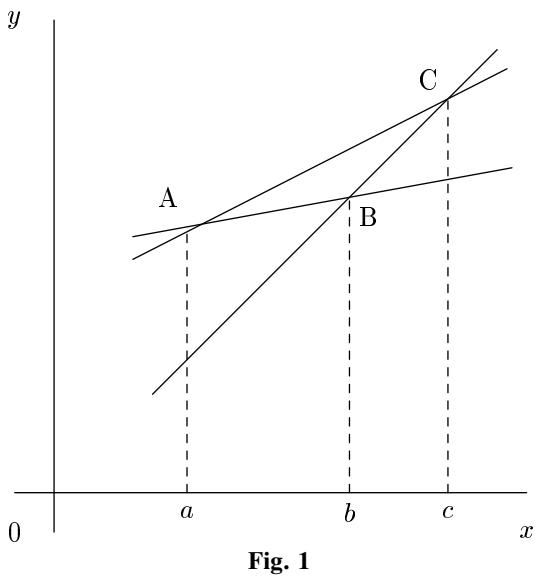
\includegraphics[keepaspectratio]{images/part001_7b60909a.jpg}}

\subsection{凸函数的定义}

定义 1. 我们说，有限数值函数 \(f\) （定义在区间 \(\mathrm{I} \subset \mathbf{R}\) 上的）在 \(\mathrm{I}\) 上是凸的，如果不论点 \(x, x'\) （\(\mathrm{I}\) 中的，\((x < x')\) ）如何，每一点 \(\mathrm{M}_z\) （属于图像 \(\mathrm{G}\) ，即 \(f\) 的图像，且满足 \(x \leqslant z \leqslant x'\) 的）都位于线段 \(\mathrm{M}_x\mathrm{M}_{x'}\) 之下（或者，等价地，如果此线段的每一点都位于 \(\mathrm{G}\) 之上）（fig.~2）。

\pandocbounded{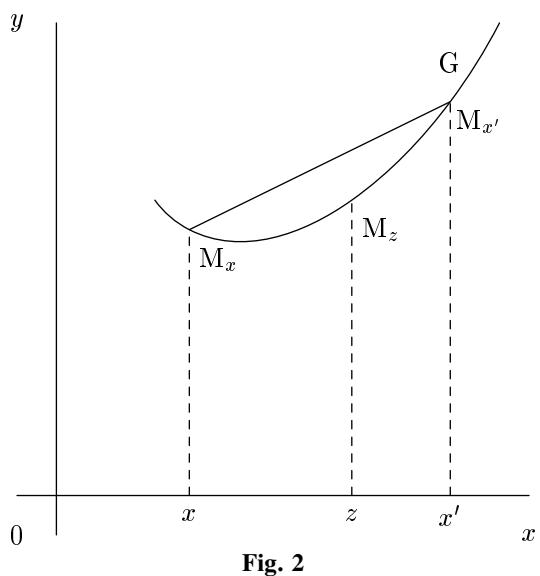
\includegraphics[keepaspectratio]{images/part001_0967d261.jpg}}

考虑到线段的参数表示（Gen.~Top., VI, p.~35），f 在 I 上凸的条件是不等式

\[
f (\lambda x + (1 - \lambda) x ^ {\prime}) \leqslant \lambda f (x) + (1 - \lambda) f (x ^ {\prime})\tag{1}
\]

对 I 的每一对点 \((x, x')\) 及每个 \(\lambda \in [0, 1]\) 成立。

定义 1 等价于：\(\mathbf{R}^2\) 中位于图像 \(G\) （即 \(f\) 的图像）上方的点所成的集是凸的。事实上，这一条件显然足以使 \(f\) 在 I 上凸；它也是必要的，因为若 \(f\) 在 I 上凸，且 \((x,y)\) 、\((x',y')\) 是位于 \(G\) 上方的两点，则有 \(y \geqslant f(x)\) ，\(y' \geqslant f(x')\) ，由此，对 \(0 \leqslant \lambda \leqslant 1\) ，

\[
\lambda y + (1 - \lambda) y ^ {\prime} \geqslant \lambda f (x) + (1 - \lambda) f \left(x ^ {\prime}\right) \geqslant f (\lambda x + (1 - \lambda) x ^ {\prime})
\]

（由 (1)），这表明以 \((x, y)\) 与 \((x', y')\) 为端点的线段的每一点都位于 G 上方。

注. 同样可以看出，严格位于 G 上方的点所成的集是凸的。反之，若此集是凸的，则有

\[
\lambda y + (1 - \lambda) y ^ {\prime} > f (\lambda x + (1 - \lambda) x ^ {\prime})
\]

对 \(0 \leqslant \lambda \leqslant 1\) 及 \(y > f(x)\) 、\(y' > f(x')\) 成立；在此公式中让 \(y\) 趋于 \(f(x)\) 、\(y'\) 趋于 \(f(x')\) ，便得出 \(f\) 是凸的。

例。1) 每个（实）仿射线性函数 \(ax + b\) 在 \(\mathbf{R}\) 上都是凸的。

\begin{enumerate}
\def\labelenumi{\arabic{enumi})}
\setcounter{enumi}{1}
\tightlist
\item
  函数 \(x^{2}\) 在 \(\mathbf{R}\) 上是凸的，因为有
\end{enumerate}

\[
\lambda x ^ {2} + (1 - \lambda) x ^ {\prime 2} - \left(\lambda x + (1 - \lambda) x ^ {\prime}\right) ^ {2} = \lambda (1 - \lambda) (x - x ^ {\prime}) ^ {2} \geqslant 0
\]

对 \(0 \leqslant \lambda \leqslant 1\) 。

\begin{enumerate}
\def\labelenumi{\arabic{enumi})}
\setcounter{enumi}{2}
\tightlist
\item
  函数 \(|x|\) 在 \(\mathbf{R}\) 上是凸的，因为
\end{enumerate}

\[
\left| \lambda x + (1 - \lambda) x ^ {\prime} \right| \leqslant \lambda | x | + (1 - \lambda) \left| x ^ {\prime} \right|
\]

对 \(0 \leqslant \lambda \leqslant 1\) 。

显然，若 \(f\) 在 \(\mathbf{I}\) 上凸，则它在任何区间 \(\mathbf{J} \subset \mathbf{I}\) 上的限制在 \(\mathbf{J}\) 上凸。

设 \(f\) 是 \(I\) 上的凸函数，\(x, x'\) 是 \(I\) 中两点，满足 \(x < x'\) ；若 \(z \in I\) 在 \([x, x']\) 之外，则 \(M_z\) 位于直线 \(D\) （联结 \(M_x\) 与 \(M_{x'}\) 的）上方；这是引理的直接推论。

由此推出：若 z 是满足 \(x < z < x'\) 的点且 \(M_{z}\) 位于线段 \(M_{x}M_{x'}\) 上，则对任何别的点 \(z'\) （满足 \(x < z' < x'\) 的），点 \(M_{z'}\) 也位于线段 \(M_{x}M_{x'}\) 上，因为由上所述 \(M_{z'}\) 同时位于此线段的上方和下方；换句话说，此时 f 在 \([x, x']\) 上等于一个仿射线性函数。

定义 2. 我们说，有限实函数 \(f\) （定义在区间 \(\mathbf{I} \subset \mathbf{R}\) 上的）在 \(\mathbf{I}\) 上是严格凸的，如果对任意点 \(x, x'\) （\(\mathbf{I}\) 中的， \(x < x'\) ），每一点 \(\mathbf{M}_z\) （属于图像 \(\mathbf{G}\) ，即 \(f\) 的图像，且满足 \(x < z < x'\) 的）都严格位于线段 \(\mathbf{M}_x\mathbf{M}_{x'}\) 之下（或者，等价地，如果此线段的每一点除端点外都严格位于 \(\mathbf{G}\) 之上）。

换句话说，必须有不等式

\[
f (\lambda x + (1 - \lambda) x ^ {\prime}) <   \lambda f (x) + (1 - \lambda) f (x ^ {\prime})\tag{2}
\]

对 I 的每一对不同的点 \((x, x')\) 及每个 \(\lambda\) （满足 \(0 < \lambda < 1\) 的）成立。

定义 2 之前的那些说明表明：为使凸函数 f 在 I 上严格凸，当且仅当不存在包含在 I 中的（不退化为一点的）区间使得 f 在其上的限制是仿射线性的。

在上面的例子中，第一个和第三个不是严格凸的；另一方面，\(x^2\) 在 \(\mathbf{R}\) 上严格凸；类似的计算表明 \(1 / x\) 在 \(]0, +\infty[\) 上严格凸。

命题 1. 设 \(f\) 是有限实函数，在区间 \(\mathbf{I} \subset \mathbf{R}\) 上凸（相应地，严格凸）。对每一家族 \((x_i)_{1 \leqslant i \leqslant p}\) （由 \(p \geqslant 2\) 个属于 \(\mathbf{I}\) 的不同的点组成），及每一家族 \((\lambda_i)_{1 \leqslant i \leqslant p}\) （由 \(p\) 个实数组成，满足 \(0 < \lambda_i < 1\) 且 \(\sum_{i=1}^{p} \lambda_i = 1\) ），我们有

\[
f \left(\sum_ {i = 1} ^ {p} \lambda_ {i} x _ {i}\right) \leqslant \sum_ {i = 1} ^ {p} \lambda_ {i} f (x _ {i})\tag{3}
\]

（相应地，

\[
f \left(\sum_ {i = 1} ^ {p} \lambda_ {i} x _ {i}\right) <   \sum_ {i = 1} ^ {p} \lambda_ {i} f (x _ {i})).\tag{4}
\]

由于该命题（就凸函数而言）在 \(p = 2\) 时归结为不等式 (1)，我们对 \(p > 2\) 用归纳法论证。数 \(\mu = \sum_{i=1}^{p-1} \lambda_i\) 为 \(> 0\) ；立即可以看出，若 \(a\) 与 \(b\) 是诸 \(x_i\) 中最小者和最大者，则 \(a \leqslant \sum_{i=1}^{p-1} \lambda_i x_i / \sum_{i=1}^{p-1} \lambda_i \leqslant b\) ；换句话说，点 \(x = \frac{1}{\mu} \sum_{i=1}^{p-1} \lambda_i x_i\) 属于 I，且归纳假设蕴含 \(\mu f(x) \leqslant \sum_{i=1}^{p-1} \lambda_i f(x_i)\) ；此外，由 (1) 我们有

\[
f \left(\sum_ {i = 1} ^ {p} \lambda_ {i} x _ {i}\right) = f (\mu x + (1 - \mu) x _ {p}) \leqslant \mu f (x) + (1 - \mu) f (x _ {p}) \leqslant \sum_ {i = 1} ^ {p} \lambda_ {i} f (x _ {i}).
\]

对严格凸函数，从不等式 (2) 出发，同样论证。

我们说有限实函数 \(f\) 在 I 上是凹的（相应地，严格凹的），如果 \(-f\) 在 I 上是凸的（相应地，严格凸的）。这等价于说，对 I 的每一对不同的点 \((x, x')\) 及每个 \(\lambda\) （满足 \(0 < \lambda < 1\) 的），有

\[
f (\lambda x + (1 - \lambda) x ^ {\prime}) \geqslant \lambda f (x) + (1 - \lambda) f (x ^ {\prime})
\]

\[
(\text { resp. } f (\lambda x + (1 - \lambda) x ^ {\prime}) > \lambda f (x) + (1 - \lambda) f (x ^ {\prime})).
\]

\subsection{凸函数族}

命题 2. 设 \(f_{i}\) （ \(1 \leqslant i \leqslant p\) ）是 \(p\) 个凸函数（定义在区间 \(\mathbf{I} \subset \mathbf{R}\) 上的），\(c_{i}\) （ \(1 \leqslant i \leqslant p\) ）是 \(p\) 个任意正数；则函数 \(f = \sum_{i=1}^{p} c_{i} f_{i}\) 在 \(\mathbf{I}\) 上凸。此外，若对至少一个指标 \(j\) ，函数 \(f_{j}\) 在 \(\mathbf{I}\) 上严格凸，且 \(c_{j} > 0\) ，则 \(f\) 在 \(\mathbf{I}\) 上严格凸。

把不等式 (1)（相应地，(2)）应用于每个 \(f_{i}\) ，把关于 \(f_{i}\) 的不等式乘以 \(c_{i}\) ，然后逐项相加，便立即得出结论。

命题 3. 设 \((f_{\alpha})\) 是区间 \(\mathbf{I} \subset \mathbf{R}\) 上的一族凸函数；若此族的上包络 \(g\) 在 \(\mathbf{I}\) 的每一点处有限，则 \(g\) 在 \(\mathbf{I}\) 上凸。

事实上，位于 g 的图像上方的点 \((x, y) \in \mathbf{R}^{2}\) 所成的集是由位于诸函数 \(f_{\alpha}\) 中每一个的图像上方的点所成的凸集之交；因此它是凸的。

命题 4. 设 H 是区间 \(I \subset R\) 上的一集凸函数；若 F 是 H 上的一个滤子，它在 I 上逐点收敛于一个有限实函数 \(f_{0}\) ，则此函数在 I 上凸。

为看出这一点，只需在不等式 (1) 中沿 F 取极限。
